\documentclass[conference]{IEEEtran}
\IEEEoverridecommandlockouts
% IEEE conference template (version 6/27/2024). All numbers in this paper are produced by
% experiments/run_experiments.py (seed 42); the raw CSV/JSON outputs are in experiments/results/.

\usepackage[T1]{fontenc}
\usepackage{cite}
\usepackage{amsmath,amssymb,amsfonts}
\usepackage{algorithmic}
\usepackage{graphicx}
\usepackage{textcomp}
\usepackage{xcolor}
\usepackage{booktabs}
\usepackage{multirow}
\usepackage{tikz}
\usetikzlibrary{shapes.geometric, arrows.meta, positioning, fit, backgrounds}
\graphicspath{{figures/}}
\def\BibTeX{{\rm B\kern-.05em{\sc i\kern-.025em b}\kern-.08em
    T\kern-.1667em\lower.7ex\hbox{E}\kern-.125emX}}

\begin{document}

\title{Auditing Fairness and Bias in Classical Machine Learning Models for Income Prediction}

\author{\IEEEauthorblockN{Saransh Gupta}
\IEEEauthorblockA{\textit{IIB2024030} \\ iib2024030@iiita.ac.in \\
\textit{Indian Institute of Information}\\ \textit{Technology, Allahabad}\\
Prayagraj, India}
\and
\IEEEauthorblockN{Sayan Samajpati}
\IEEEauthorblockA{\textit{IIB2024013} \\ iib2024013@iiita.ac.in \\
\textit{Indian Institute of Information}\\ \textit{Technology, Allahabad}\\
Prayagraj, India}
\and
\IEEEauthorblockN{Ayush Anand}
\IEEEauthorblockA{\textit{IIT2024246} \\ iit2024246@iiita.ac.in \\
\textit{Indian Institute of Information}\\ \textit{Technology, Allahabad}\\
Prayagraj, India}
\and
\IEEEauthorblockN{Adabala Sridhar}
\IEEEauthorblockA{\textit{IIT2024218} \\ iit2024218@iiita.ac.in \\
\textit{Indian Institute of Information}\\ \textit{Technology, Allahabad}\\
Prayagraj, India}
}

\maketitle

%% ------------------------------------------------------------------
\begin{abstract}
Classifiers used to support income and credit decisions are usually judged by aggregate accuracy, which can hide systematic differences in how demographic groups are treated. We audit four classical machine learning models---logistic regression, linear SVM, random forest and gradient boosting---on the UCI Adult census income dataset (48{,}790 records after cleaning) and measure group fairness with respect to sex, race and age group using the demographic parity (DP), equal opportunity (EO), false positive rate and predictive parity gaps, plus an intersectional sex$\times$race audit. Every gap is validated with bootstrap confidence intervals and $z$/$\chi^2$ tests. All four models are significantly biased: the strongest model (gradient boosting, 87.0\% accuracy, F1 0.707) predicts a high income for 26.4\% of men but only 8.3\% of women (DP gap 0.181, 95\% CI [0.168, 0.194], $p<10^{-10}$). Removing sex and race from the inputs (``fairness through unawareness'') leaves the sex gap practically unchanged (0.171), showing that proxy features carry the bias. Five mitigation methods spanning pre-, in- and post-processing are compared: reweighing cuts the DP gap to 0.101 for 0.6 accuracy points, the disparate impact remover barely helps, exponentiated-gradient in-processing can drive the DP gap to 0.023 but at 2.4 accuracy points and a large EO cost, group-specific thresholds remove the EO gap (0.075$\rightarrow$0.002) for 0.2 points, and equalized-odds post-processing equalizes TPR and FPR together for 1.6 points. Training and validation loss curves confirm convergence. The results reproduce the accuracy--fairness trade-off and the incompatibility of fairness criteria: no method improves every gap at once.
\end{abstract}

\begin{IEEEkeywords}
algorithmic fairness, bias mitigation, income prediction, classical machine learning, demographic parity, equal opportunity, reweighing
\end{IEEEkeywords}

%% ------------------------------------------------------------------
\section{Introduction and Related Work}
\subsection{Introduction}
Machine learning models now routinely support decisions about loans, credit and hiring. Fitted to historical data, they can reproduce the inequalities recorded in that data, and a single accuracy number says nothing about whether this happens. Regulators increasingly require evidence that a model does not disadvantage protected groups, and classical models remain the industry standard in lending because they are interpretable and auditable.

In this project we treat fairness auditing as a first-class part of model evaluation on the standard income prediction benchmark, the UCI Adult dataset. We ask three questions: (1) how large are the disparities between demographic groups in the predictions of standard classical models, (2) are those disparities statistically significant or just noise from small groups, and (3) how much fairness can be gained by established mitigation methods and at what cost in accuracy?

Our contributions are: (i) a fully reproducible audit pipeline (single seed, leakage-free preprocessing, train/validation/test protocol) covering four classical models; (ii) a statistical validation of every fairness gap with bootstrap confidence intervals and hypothesis tests; (iii) three ablation studies---with versus without the sensitive attributes, across model families, and before versus after mitigation; and (iv) a before/after comparison of five mitigation methods covering all three intervention families (reweighing and disparate impact removal; exponentiated-gradient reductions; group thresholds and equalized-odds post-processing).

\subsection{Related Work}
\textbf{Fairness definitions.} Group fairness criteria compare a statistic of the classifier across groups defined by a sensitive attribute: demographic parity asks for equal positive prediction rates~\cite{dwork2012}, equality of opportunity for equal true positive rates and equalized odds additionally for equal false positive rates~\cite{hardt2016}, predictive parity for equal precision~\cite{chouldechova2017}. These criteria are mutually incompatible when base rates differ~\cite{kleinberg2017,chouldechova2017}, so an audit must report several of them.

\textbf{Bias and mitigation.} Surveys~\cite{mehrabi2021,pessach2022,barocas2023} catalogue the sources of bias and three families of mitigation. Pre-processing: reweighing~\cite{calders2009,kamiran2012} weights training records so that group and label become independent; the disparate impact remover~\cite{feldman2015} repairs feature distributions. In-processing: the reductions approach~\cite{agarwal2018} turns a fairness constraint into a sequence of cost-sensitive problems for any base learner. Post-processing: Hardt \textit{et al.}~\cite{hardt2016} choose (randomized) group-specific decision rules on a fixed scorer. Friedler \textit{et al.}~\cite{friedler2019} showed that results depend strongly on preprocessing and the split, which motivates our strict seeding and confidence intervals.

\textbf{Credit scoring and the Adult dataset.} Kozodoi \textit{et al.}~\cite{kozodoi2022} and Thu \textit{et al.}~\cite{thu2026} evaluate fairness-aware learning on credit data and find fairness gains at modest profit cost; we follow their protocol of combining classical models with all three mitigation families. Adult~\cite{kohavi1996,dua2019} is the most used fairness benchmark; Ding \textit{et al.}~\cite{ding2021} discuss its limitations, which we revisit in the conclusion.

%% ------------------------------------------------------------------
\section{Methodology}
\subsection{System Architecture}
Fig.~\ref{fig:method} shows the pipeline. The census table is cleaned, explored and split once into training, validation and test sets. All preprocessing is fitted on the training split only, inside a scikit-learn~\cite{pedregosa2011} \texttt{Pipeline}, so nothing can leak from validation or test data. Four classical classifiers are tuned by cross-validation and evaluated on the test split; their predictions go through a fairness audit (per-group rates, gaps, bootstrap uncertainty, significance tests). Finally five mitigation methods are applied to two representative models and the audit is repeated on identical test records.

\begin{figure}[t]
\centering
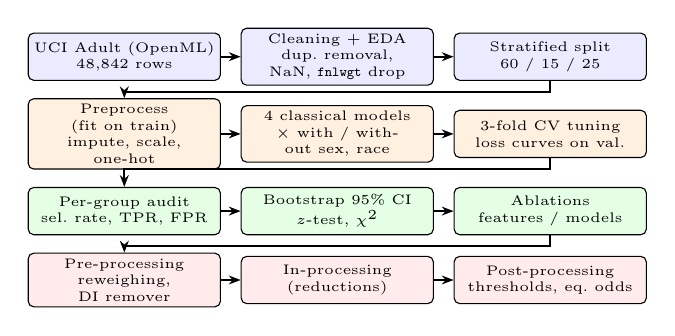
\begin{tikzpicture}[
  node distance=0.22cm and 0.25cm,
  box/.style={rectangle, draw, rounded corners=2pt, text width=2.3cm, minimum height=0.6cm, align=center, font=\tiny, inner sep=2pt, fill=white},
  data/.style={box, fill=blue!8},
  model/.style={box, fill=orange!12},
  audit/.style={box, fill=green!10},
  mit/.style={box, fill=red!8},
  arr/.style={-{Stealth[length=1.5mm]}, thick}]
\node[data] (raw) {UCI Adult (OpenML)\\48{,}842 rows};
\node[data, right=of raw] (clean) {Cleaning + EDA\\dup.\ removal, NaN, \texttt{fnlwgt} drop};
\node[data, right=of clean] (split) {Stratified split\\60 / 15 / 25};
\node[model, below=of raw] (prep) {Preprocess (fit on train)\\impute, scale, one-hot};
\node[model, right=of prep] (train) {4 classical models\\$\times$ with / without sex, race};
\node[model, right=of train] (tune) {3-fold CV tuning\\loss curves on val.};
\node[audit, below=of prep] (metrics) {Per-group audit\\sel.\ rate, TPR, FPR};
\node[audit, right=of metrics] (stats) {Bootstrap 95\% CI\\$z$-test, $\chi^2$};
\node[audit, right=of stats] (ablate) {Ablations\\features / models};
\node[mit, below=of metrics] (rw) {Pre-processing\\reweighing, DI remover};
\node[mit, right=of rw] (th) {In-processing\\(reductions)};
\node[mit, right=of th] (cmp) {Post-processing\\thresholds, eq.\ odds};
\draw[arr] (raw) -- (clean); \draw[arr] (clean) -- (split);
\draw[arr] (split.south) -- ++(0,-0.14) -| (prep.north);
\draw[arr] (prep) -- (train); \draw[arr] (train) -- (tune);
\draw[arr] (tune.south) -- ++(0,-0.14) -| (metrics.north);
\draw[arr] (metrics) -- (stats); \draw[arr] (stats) -- (ablate);
\draw[arr] (ablate.south) -- ++(0,-0.14) -| (rw.north);
\draw[arr] (rw) -- (th); \draw[arr] (th) -- (cmp);
\end{tikzpicture}
\caption{System architecture and workflow. Blue: data stage, orange: modelling stage, green: fairness audit, red: mitigation.}
\label{fig:method}
\end{figure}

\subsection{Dataset}
We use the UCI Adult (Census Income) dataset~\cite{kohavi1996,dua2019}, loaded from OpenML (\texttt{adult}, version~2). It contains 48{,}842 records extracted from the 1994 US census, 14 attributes and the binary target ``income $>$ 50K''. Table~\ref{tab:data} summarizes the data and Table~\ref{tab:sample} shows representative rows. The sensitive attributes are \texttt{sex} (binary in this data), \texttt{race} (five categories) and, following the proposal, an \texttt{age group} derived from age ($<$30, 30--44, 45--59, 60+). The other features are age, workclass, education and education-num, marital status, occupation, relationship, capital gain and loss, hours per week and native country. The class is imbalanced (23.9\% positive), so F1 and per-group true positive rates matter more than accuracy alone.

In the OpenML version the ``?'' placeholders are already stored as missing values (workclass 2{,}795, occupation 2{,}805, native-country 856 missing). White space is stripped, 52 exact duplicate rows are dropped (leaving 48{,}790 rows) and the census sampling weight \texttt{fnlwgt} is removed because it is not a personal attribute. Missing values are imputed inside the pipeline (median for numeric, most frequent for categorical). The bias is already in the labels: 30.4\% of men but 10.9\% of women earn more than 50K, the rate ranges from 11.7\% (Amer-Indian-Eskimo) to 27.0\% (Asian-Pac-Islander) across race groups and from 5.4\% ($<$30) to 38.8\% (45--59) across age groups.

\begin{table}[t]
\caption{Dataset summary after cleaning.}
\label{tab:data}
\centering\scriptsize
\begin{tabular}{ll}
\toprule
Source & UCI / OpenML \texttt{adult} v2 (1994 US census) \\
Records & 48{,}842 raw $\rightarrow$ 48{,}790 after removing 52 duplicates \\
Features used & 13 (5 numeric, 8 categorical); \texttt{fnlwgt} dropped \\
Target & income $>$ 50K: 23.9\% positive, 76.1\% negative \\
Sex & Male 32{,}614 (66.8\%), Female 16{,}176 (33.2\%) \\
Race & White 41{,}714; Black 4{,}683; Asian-Pac-Isl.\ 1{,}517; \\
     & Amer-Indian-Eskimo 470; Other 406 \\
Missing & workclass 5.7\%, occupation 5.7\%, native-country 1.8\% \\
\bottomrule
\end{tabular}
\end{table}

\begin{table}[t]
\caption{Five representative records (random sample, seed 42).}
\label{tab:sample}
\centering\scriptsize
\setlength{\tabcolsep}{3pt}
\begin{tabular}{rlllllrl}
\toprule
age & workclass & education & marital & occupation & race/sex & hrs & class \\
\midrule
54 & State-gov & Some-college & Married & Adm-clerical & White/M & 40 & $\leq$50K \\
43 & Private & Bachelors & Divorced & Sales & White/M & 44 & $>$50K \\
29 & Private & Bachelors & Never-marr. & Prof-specialty & White/M & 45 & $>$50K \\
47 & Private & Bachelors & Married & Sales & Black/M & 40 & $>$50K \\
46 & Private & HS-grad & Divorced & Protective-serv & White/M & 40 & $\leq$50K \\
\bottomrule
\end{tabular}
\end{table}

\subsection{Dataset Division}
The cleaned data is split once with a fixed seed (42), stratified on the label. First 25\% is held out as the test set; the remaining 75\% is split 80/20 into training and validation sets. This gives 29{,}273 training (60\%), 7{,}319 validation (15\%) and 12{,}198 test records (25\%), each with 23.9\% positives. Training is used for CV tuning and fitting, validation only for loss curves and for fitting the post-processing rules, and the test set is touched once per final model. The test set contains 8{,}194 men and 4{,}004 women, and 10{,}459 White, 1{,}152 Black, 367 Asian-Pac-Islander, 116 Amer-Indian-Eskimo and 104 Other records; by age group 3{,}607 / 4{,}688 / 2{,}864 / 1{,}039 ($<$30 / 30--44 / 45--59 / 60+). The three smallest race groups are small.

\subsection{Models}
Following the proposal we train four classical classifiers: $\ell_2$-regularized logistic regression, a linear support vector machine (\texttt{LinearSVC}), a random forest and histogram-based gradient boosting (\texttt{HistGradientBoostingClassifier}). Each is trained in two variants: \emph{with} the sensitive attributes among the inputs, and \emph{without} them (sex and race removed, ``fairness through unawareness''). No deep learning is used.

\subsection{Fairness Metrics}
For a group $g$, prediction $\hat{y}$ and label $y$ we compute on the test set the selection rate $\mathrm{SR}_g = P(\hat{y}=1\mid g)$, the true positive rate $\mathrm{TPR}_g = P(\hat{y}=1\mid y=1,g)$ and the false positive rate $\mathrm{FPR}_g = P(\hat{y}=1\mid y=0,g)$. The demographic parity gap is $\Delta_{\mathrm{DP}}=\max_g \mathrm{SR}_g-\min_g \mathrm{SR}_g$, the equal opportunity gap is $\Delta_{\mathrm{EO}}=\max_g \mathrm{TPR}_g-\min_g \mathrm{TPR}_g$~\cite{hardt2016}, and the FPR gap is defined analogously (together with $\Delta_{\mathrm{EO}}$ it measures equalized odds). We also report the predictive parity gap, the range of the positive predictive value $\mathrm{PPV}_g=P(y=1\mid\hat{y}=1,g)$ across groups~\cite{chouldechova2017}. A gap of 0 is perfectly fair under that criterion. Gaps are computed for sex, race, age group and for the ten intersectional sex$\times$race groups.

\subsection{Statistical Validation}
A gap measured on a finite test set is itself a random quantity. We therefore (i) resample the test set with replacement 1{,}000 times and report the 2.5th and 97.5th percentiles of each gap as a 95\% bootstrap confidence interval, and (ii) test the null hypothesis of equal selection rates with a two-proportion $z$-test (Male vs.\ Female, White vs.\ Black) and a $\chi^2$ test of independence between group and prediction, at $\alpha=0.05$.

\subsection{Bias Mitigation}
\textbf{Reweighing (pre-processing)~\cite{kamiran2012}.} Each training record with group $g$ and label $y$ receives the weight $w(g,y)=P(g)P(y)/P(g,y)$, so that in the weighted training set the group and the label are independent. On our training split the weights are 2.17 for high-income women, 0.85 for low-income women, 0.79 for high-income men and 1.09 for low-income men. The classifier is refitted with these sample weights; the inputs still exclude sex and race.

\textbf{Group-specific thresholds (post-processing)~\cite{hardt2016}.} The unmitigated scorer is kept, but the 0.5 decision threshold is replaced by one threshold per group. The thresholds are chosen on the \emph{validation} split so that every group reaches the same TPR as the overall validation TPR at 0.5, and are then applied unchanged to the test split. For gradient boosting this gives thresholds of 0.513 for men and 0.412 for women. We also evaluate the two methods combined.

\textbf{Disparate impact remover (pre-processing)~\cite{feldman2015}.} Each numeric feature is repaired so that its distribution no longer differs between sexes: a value at within-group quantile $q$ is replaced by the value at quantile $q$ of the median distribution across groups (repair level $\lambda=1$, 101 quantiles fitted on the training split; categorical features unchanged). The classifier is retrained on the repaired features.

\textbf{Exponentiated-gradient reductions (in-processing)~\cite{agarwal2018}.} A demographic parity or equalized odds constraint (violation $\epsilon=0.01$) is enforced by a saddle-point algorithm that repeatedly refits the tuned base learner on reweighted, relabelled data and returns a randomized ensemble of 12--21 classifiers (\texttt{fairlearn} implementation).

\textbf{Equalized-odds post-processing~\cite{hardt2016}.} \texttt{fairlearn}'s \texttt{ThresholdOptimizer} finds on the validation split group-specific randomized thresholds that equalize TPR and FPR while maximizing accuracy; the rule is then applied to the test split.

%% ------------------------------------------------------------------
\section{Experimental Settings}
\textbf{Hardware and software.} All experiments run on CPU on an Apple M4 laptop with 16~GB RAM (the complete pipeline takes about 90 seconds and also runs on a free Google Colab instance). Software: Python 3.12.13, scikit-learn 1.9.1, fairlearn 0.15.0, NumPy 2.5.4, pandas 3.1.1, SciPy 1.18.1, Matplotlib 3.11. All random components use seed 42.

\textbf{Preprocessing.} Numeric features: median imputation and standardization. Categorical features: most-frequent imputation and one-hot encoding (unknown categories ignored), producing 104 input columns with and 97 without the sensitive attributes.

\textbf{Hyperparameters.} Each model is tuned by grid search with 3-fold stratified cross-validation on the training split, maximizing F1 (Table~\ref{tab:hyper}). The validation accuracy of the selected configuration is also reported as a sanity check.

\begin{table}[t]
\caption{Hyperparameter grids (3-fold CV, F1) and selected values.}
\label{tab:hyper}
\centering\scriptsize
\setlength{\tabcolsep}{3pt}
\begin{tabular}{lll}
\toprule
Model & Grid & Selected (with / without) \\
\midrule
Logistic regr. & $C\in\{0.01,0.1,1,10\}$, lbfgs, 2000 it. & $C{=}10$ / $C{=}1$ \\
Linear SVM & $C\in\{0.01,0.1,1\}$, 5000 it. & $C{=}1$ / $C{=}1$ \\
Random forest & 200 trees, depth $\{10,20,\infty\}$, & depth 20, \\
 & min leaf $\{1,5\}$ & min leaf 1 (both) \\
Gradient boost. & lr $\{0.05,0.1\}$, iters $\{200,400\}$, & lr 0.1, 200 it., \\
 & leaves $\{15,31\}$ & 31 leaves (both) \\
\bottomrule
\end{tabular}
\end{table}

\textbf{Loss curves.} Random forests and SVMs have no notion of an epoch, so loss curves are produced for the two iteratively fitted models: logistic regression by stochastic gradient descent (\texttt{SGDClassifier}, log loss, $\alpha=10^{-4}$, one shuffled pass per epoch, 40 epochs) and gradient boosting (log loss after each of 400 iterations, no early stopping), recording training and validation log loss at every step.

%% ------------------------------------------------------------------
\section{Results and Ablation Studies}

\subsection{Training and Validation Loss}
Fig.~\ref{fig:loss} shows the loss curves. For SGD logistic regression (a) the training log loss falls from 0.518 after the first epoch to 0.322 after 40 epochs and the validation loss from 0.547 to 0.324; the two curves move together and the validation loss reaches its minimum (0.321) at epoch 34, so the linear model converges without overfitting (validation accuracy 85.5\%, matching the lbfgs solution). For gradient boosting (b) the training loss keeps decreasing to 0.203 at iteration 400, but the validation loss reaches its minimum of 0.278 at iteration 120 and then slowly rises to 0.286: beyond roughly 100--200 iterations the ensemble starts to memorize the training set. This agrees with the cross-validation choice of 200 iterations rather than 400, and it is the expected signature of mild overfitting in a boosted ensemble.

\begin{figure*}[t]
\centering
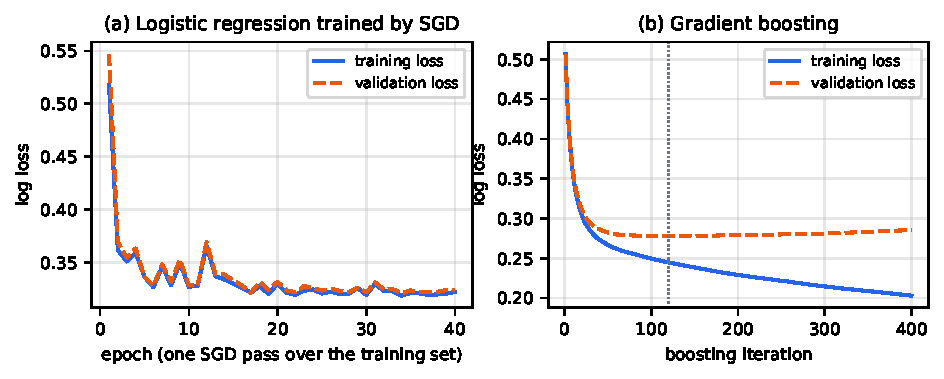
\includegraphics[width=0.78\textwidth]{loss_curve.pdf}
\caption{Training and validation loss. (a) Logistic regression trained by SGD: log loss per epoch. (b) Gradient boosting: log loss per boosting iteration; the dotted line marks the minimum validation loss (iteration 120).}
\label{fig:loss}
\end{figure*}

\subsection{Performance Metrics}
Table~\ref{tab:main} reports test-set accuracy, precision, recall, F1 and ROC-AUC for all eight models with the fairness gaps. Gradient boosting is the strongest predictor (87.0\% accuracy, F1 0.707, AUC 0.925; confusion matrix 8{,}699 TN, 1{,}913 TP, 579 FP, 1{,}007 FN), followed by random forest (86.1\%); the linear models are 1.8 points lower. Precision (0.74--0.78) exceeds recall (0.57--0.66) everywhere: all models miss many true high earners. Tree ensembles win on raw accuracy, as the proposal expected.

\begin{table*}[t]
\caption{Test-set performance and fairness gaps of all models (12{,}198 records). DP = demographic parity gap, EO = equal opportunity gap. ``with''/``without'' refers to sex and race being input features.}
\label{tab:main}
\centering\scriptsize
\begin{tabular}{llccccc|ccc|ccc}
\toprule
 & & \multicolumn{5}{c|}{Overall performance} & \multicolumn{3}{c|}{Gaps by sex} & \multicolumn{3}{c}{Gaps by race} \\
Model & Variant & Acc. & Prec. & Rec. & F1 & AUC & DP & EO & FPR & DP & EO & FPR \\
\midrule
Logistic regression & with & 0.852 & 0.739 & 0.593 & 0.658 & 0.904 & 0.180 & 0.119 & 0.071 & 0.241 & 0.376 & 0.119 \\
 & without & 0.852 & 0.739 & 0.587 & 0.655 & 0.903 & 0.174 & 0.099 & 0.067 & 0.198 & 0.174 & 0.119 \\
Linear SVM & with & 0.852 & 0.747 & 0.578 & 0.652 & 0.903 & 0.172 & 0.111 & 0.065 & 0.233 & 0.367 & 0.112 \\
 & without & 0.850 & 0.743 & 0.572 & 0.646 & 0.902 & 0.164 & 0.081 & 0.061 & 0.193 & 0.159 & 0.119 \\
Random forest & with & 0.861 & 0.774 & 0.591 & 0.670 & 0.914 & 0.160 & 0.073 & 0.052 & 0.200 & 0.312 & 0.101 \\
 & without & 0.860 & 0.777 & 0.584 & 0.667 & 0.914 & 0.159 & 0.079 & 0.051 & 0.194 & 0.174 & 0.097 \\
Gradient boosting & with & \textbf{0.870} & 0.768 & \textbf{0.655} & \textbf{0.707} & \textbf{0.925} & 0.181 & 0.091 & 0.060 & 0.220 & 0.327 & 0.109 \\
 & without & \textbf{0.871} & 0.777 & 0.646 & 0.705 & 0.925 & 0.171 & 0.075 & 0.052 & 0.198 & 0.125 & 0.104 \\
\bottomrule
\end{tabular}
\end{table*}

\subsection{Fairness Audit}
Every model is biased by sex and by race under every criterion (Table~\ref{tab:main}). Table~\ref{tab:groups} breaks the best model down by group. Gradient boosting predicts a high income for 26.4\% of men but 8.3\% of women, a DP gap of 0.181; among people who truly earn more than 50K it finds 66.8\% of the men but only 57.7\% of the women (EO gap 0.091), and its false positive rate is 3.4 times higher for men. Per-group \emph{accuracy} is nevertheless higher for women (93.3\% vs.\ 83.9\%) because far fewer women are positive: accuracy alone would suggest the model treats women better, exactly the blind spot the audit exposes. By race, the selection rate ranges from 6.0\% (Amer-Indian-Eskimo) to 28.1\% (Asian-Pac-Islander), and the Black group is selected at 8.5\% against 21.8\% for the White group.

\textbf{Predictive parity.} The PPV gap by sex is small for every model (0.03--0.07; gradient boosting: PPV 0.774 for men, 0.725 for women): a positive prediction is about equally reliable for both sexes. This is the one criterion the unmitigated models nearly satisfy and, as Section~\ref{sec:mit} shows, exactly the one that breaks when TPR or selection rates are equalized~\cite{chouldechova2017,kleinberg2017}.

\textbf{Age group.} Age produces the largest gaps of all attributes (Fig.~\ref{fig:age}): gradient boosting selects 2.7\% of people under 30 but 34.9\% of the 45--59 group (DP gap 0.321, CI [0.304, 0.338]), and its TPR ranges from 0.389 ($<$30) to 0.699 (EO gap 0.311); the pattern is the same for all models (DP 0.26--0.32, all $\chi^2$ $p<10^{-10}$). Much of this follows the true base rates (5.4\% vs.\ 38.8\%), but the EO gap shows that young high earners are also systematically missed.

\textbf{Intersectional groups.} Splitting by sex$\times$race widens the disparity: among groups with at least 100 test records, gradient boosting selects 35.5\% of Asian-Pac-Islander men but 4.3\% of Black women (DP gap 0.312), and the TPR of Asian-Pac-Islander women (0.40, $n$=116) is far below that of White men (0.67). Black women have the lowest selection rate although their PPV is the highest (0.79): the model is most conservative where it is most often right.

\begin{figure}[t]
\centering
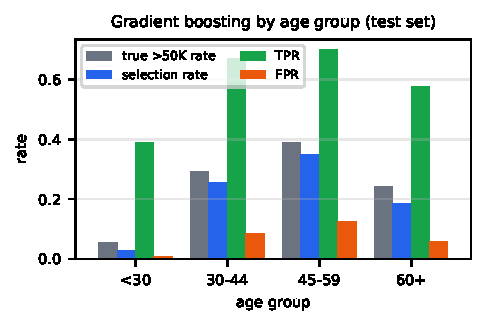
\includegraphics[width=0.72\columnwidth]{age_groups.pdf}
\caption{Gradient boosting by age group on the test set: true share of $>$50K labels, selection rate, TPR and FPR.}
\label{fig:age}
\end{figure}

\textbf{Significance.} The 95\% bootstrap intervals of the sex DP gaps are narrow (width $\approx$0.025) and far from zero for all eight models; for gradient boosting without sensitive features the DP gap is 0.171 [0.158, 0.184] and the EO gap 0.075 [0.025, 0.121]. The two-proportion $z$-test on Male vs.\ Female selection rates gives $z$ between 21.5 and 23.7 for every model, and the $\chi^2$ test of independence between group and prediction gives $\chi^2>459$ by sex (1 d.o.f.) and $\chi^2>112$ by race (4 d.o.f.); all $p$-values are below $10^{-10}$. The disparities are therefore real, not sampling noise. For race, the EO intervals are much wider (e.g.\ [0.08, 0.51] for gradient boosting without sensitive features) because the extreme groups contain only 104--116 test records, so the exact size of the race EO gap is uncertain even though its existence is not.

\begin{table}[t]
\caption{Per-group metrics of gradient boosting (with sensitive features) on the test set.}
\label{tab:groups}
\centering\scriptsize
\begin{tabular}{lrcccc}
\toprule
Group & $n$ & Sel.\ rate & TPR & FPR & Accuracy \\
\midrule
Male & 8{,}194 & 0.264 & 0.668 & 0.086 & 0.839 \\
Female & 4{,}004 & 0.083 & 0.577 & 0.025 & 0.933 \\
\midrule
White & 10{,}459 & 0.218 & 0.661 & 0.066 & 0.864 \\
Black & 1{,}152 & 0.085 & 0.589 & 0.022 & 0.935 \\
Asian-Pac-Islander & 367 & 0.281 & 0.645 & 0.131 & 0.804 \\
Amer-Indian-Eskimo & 116 & 0.060 & 0.333 & 0.029 & 0.905 \\
Other & 104 & 0.087 & 0.538 & 0.022 & 0.923 \\
\bottomrule
\end{tabular}
\end{table}

\subsection{Ablation 1: With versus Without Sensitive Attributes}
Removing sex and race from the inputs costs essentially no accuracy (at most 0.2 points, and gradient boosting even gains 0.1) but it does not make the models fair. The sex DP gap moves only from 0.180 to 0.174 (logistic regression) and from 0.181 to 0.171 (gradient boosting), and the EO gap by sex drops by 1--3 points. Marital status, relationship (``Husband''/``Wife''), occupation and hours per week are strong proxies for sex, so the model recovers it. The one place where unawareness helps substantially is the \emph{race EO gap}, which falls from 0.33--0.38 to 0.13--0.17: the tiny race categories were being used almost directly as features, and removing them stops the model from assigning a very low TPR to the Amer-Indian-Eskimo group (0.33 $\rightarrow$ 0.58).

\subsection{Ablation 2: Across Model Families}
Fairness does not follow accuracy: random forest has the smallest sex gaps (DP 0.160, EO 0.073) although gradient boosting, with the largest DP gap (0.181), is more accurate. The spread of DP gaps across the eight models (0.159--0.181) is small compared to the gap itself, so switching the classifier cannot remove the disparity; it is carried by the data and the label, matching Friedler \textit{et al.}~\cite{friedler2019}.

\subsection{Ablation 3: Before versus After Mitigation}\label{sec:mit}
Table~\ref{tab:mit} compares all mitigation methods on gradient boosting and logistic regression, starting from the ``without sensitive features'' variant.

\textbf{Reweighing} attacks demographic parity: for gradient boosting the DP gap by sex falls from 0.171 to 0.101 (95\% CI [0.088, 0.114]) and the FPR gap practically vanishes (0.052 $\rightarrow$ 0.003), because the selection rate of women rises from 8.4\% to 12\% and that of men falls from 25.5\% to 22\%. The price is 0.6 accuracy points and 2.1 F1 points, and the EO gap does not improve: it even flips sign (women's TPR 0.69 vs.\ men's 0.60) because reweighing pushes the whole female score distribution up. For logistic regression the effect is stronger in both directions (DP 0.174 $\rightarrow$ 0.083, accuracy $-1.0$ point, EO gap worse at 0.146).

\textbf{Group thresholds} attack equal opportunity: the EO gap of gradient boosting drops from 0.075 to 0.002 (95\% CI [0.001, 0.055]) with both groups at a TPR of 0.64, for only 0.2 accuracy points and 0.5 F1 points. The DP gap improves moderately (0.171 $\rightarrow$ 0.147) because equalizing the TPR still leaves the groups with different base rates. The thresholds transfer well from validation to test.

\textbf{Combination.} Thresholds on top of the reweighed model give an intermediate solution (DP 0.134, EO 0.023, accuracy 86.8\%).

\textbf{Disparate impact remover.} Repairing the numeric features changes almost nothing for gradient boosting (DP 0.173, accuracy $-1.0$ point) and only a little for logistic regression (DP 0.154): on this data the sex proxies are \emph{categorical} (relationship, marital status, occupation), which the method does not touch. It is the least effective intervention here.

\textbf{Equalized-odds post-processing.} The Hardt \textit{et al.} rule equalizes TPR \emph{and} FPR by sex (gradient boosting: EO 0.004, FPR gap 0.009, DP 0.099) at 1.6 accuracy points. The price appears elsewhere: the female FPR rises from 0.026 to 0.069 and the PPV gap jumps from 0.07 to 0.31 (0.81 for men vs.\ 0.50 for women), so a positive prediction for a woman becomes a coin flip.

\textbf{In-processing.} The exponentiated-gradient reduction with a demographic parity constraint is the only method that nearly closes the DP gap (0.023, CI [0.010, 0.036]), but only by cutting the male selection rate to 17\% and raising the female TPR to 0.745 against 0.481 for men (EO gap 0.264 in the opposite direction), at 2.4 accuracy and 8.6 F1 points. With an equalized-odds constraint it behaves like the Hardt post-processing (EO 0.037, FPR 0.014) at a smaller accuracy cost (1.0 point) but again with a PPV gap of 0.25.

Fig.~\ref{fig:tradeoff} places all configurations in the accuracy--fairness plane. Every point that improves fairness lies below the unmitigated gradient boosting point, so there is no free lunch; the cheapest Pareto moves are the simple group thresholds (for EO) and reweighing (for DP). The stronger methods reach smaller gaps on their target criterion at a higher accuracy cost and by violating predictive parity, which is the impossibility result of~\cite{kleinberg2017,chouldechova2017} observed empirically.

\begin{table}[t]
\caption{Before/after mitigation (test set, gaps by sex, 95\% bootstrap CI in brackets, last column: FPR gap / PPV gap). Pre: pre-processing, In: in-processing, Post: post-processing. Mitigation starts from the ``without sex/race'' variant.}
\label{tab:mit}
\centering\tiny
\setlength{\tabcolsep}{2.5pt}
\begin{tabular}{llccccc}
\toprule
Model & Setting & Acc. & F1 & DP gap [CI] & EO gap [CI] & FPR / PPV \\
\midrule
\multirow{9}{*}{\shortstack[l]{Gradient\\boosting}}
 & with sex/race & 0.870 & 0.707 & 0.181\,[.17,.19] & 0.091\,[.04,.14] & .060 / .049 \\
 & without sex/race & 0.871 & 0.705 & 0.171\,[.16,.18] & 0.075\,[.03,.12] & .052 / .068 \\
 & Pre: reweighing & 0.865 & 0.684 & 0.101\,[.09,.11] & 0.098\,[.04,.14] & .003 / .185 \\
 & Pre: DI remover & 0.861 & 0.682 & 0.173\,[.16,.19] & 0.066\,[.02,.12] & .063 / .033 \\
 & In: EG (DP) & 0.847 & 0.619 & \textbf{0.023}\,[.01,.04] & 0.264\,[.22,.30] & .045 / .339 \\
 & In: EG (EO) & 0.861 & 0.685 & 0.131\,[.12,.14] & 0.037\,[.00,.09] & .014 / .251 \\
 & Post: group thresholds & 0.868 & 0.701 & 0.147\,[.13,.16] & \textbf{0.002}\,[.00,.05] & .036 / .133 \\
 & Post: eq.\ odds (Hardt) & 0.855 & 0.661 & 0.099\,[.09,.11] & 0.004\,[.00,.06] & .009 / .312 \\
 & reweighing + thresholds & 0.868 & 0.690 & 0.134\,[.12,.15] & 0.023\,[.00,.07] & .029 / .176 \\
\midrule
\multirow{9}{*}{\shortstack[l]{Logistic\\regression}}
 & with sex/race & 0.852 & 0.658 & 0.180\,[.17,.19] & 0.119\,[.06,.17] & .071 / .029 \\
 & without sex/race & 0.852 & 0.655 & 0.174\,[.16,.19] & 0.099\,[.05,.15] & .067 / .035 \\
 & Pre: reweighing & 0.842 & 0.622 & 0.083\,[.07,.10] & 0.146\,[.09,.19] & .007 / .161 \\
 & Pre: DI remover & 0.848 & 0.643 & 0.154\,[.14,.17] & 0.040\,[.00,.10] & .057 / .064 \\
 & In: EG (DP) & 0.830 & 0.569 & \textbf{0.015}\,[.00,.03] & 0.271\,[.22,.32] & .040 / .321 \\
 & In: EG (EO) & 0.838 & 0.605 & 0.101\,[.09,.11] & \textbf{0.000}\,[.00,.06] & .011 / .251 \\
 & Post: group thresholds & 0.847 & 0.644 & 0.131\,[.12,.14] & 0.036\,[.00,.08] & .041 / .105 \\
 & Post: eq.\ odds (Hardt) & 0.834 & 0.622 & 0.097\,[.08,.11] & 0.011\,[.00,.06] & .000 / .305 \\
 & reweighing + thresholds & 0.847 & 0.629 & 0.132\,[.12,.14] & 0.004\,[.00,.06] & .042 / .136 \\
\bottomrule
\end{tabular}
\end{table}

\begin{figure}[t]
\centering
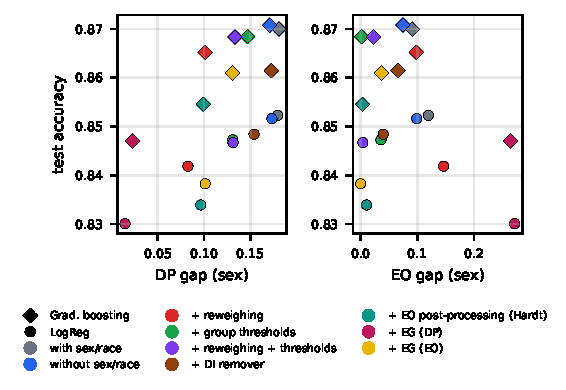
\includegraphics[width=0.84\columnwidth]{tradeoff_ext.pdf}
\caption{Accuracy--fairness trade-off of all mitigation configurations for gradient boosting (diamonds) and logistic regression (circles); colour: setting. Top-left is best. Group thresholds and reweighing give the cheapest improvements; in-processing with a DP constraint reaches the smallest DP gap at the largest accuracy cost.}
\label{fig:tradeoff}
\end{figure}

%% ------------------------------------------------------------------
\section{Conclusion}
We audited four classical classifiers on the Adult income task with a leakage-free, seeded train/validation/test protocol. All are strongly and significantly biased: the best model (gradient boosting, 87.0\% accuracy, F1 0.707) selects men 3.2 times as often as women (DP gap 0.181, $p<10^{-10}$) and misses 9 points more of the truly high-earning women (EO gap 0.091), while per-group accuracy would suggest the opposite. First, removing the sensitive attributes is nearly free but nearly useless for the sex disparity (gap 0.171) because other features act as proxies. Second, the model family changes the gap by only two points: the bias is in the data, not the learner. Third, age produces even larger gaps (DP 0.32) and intersectional groups larger still (DP 0.31 between Asian-Pac-Islander men and Black women). Fourth, mitigation works but is criterion-specific: reweighing cuts the demographic parity gap by 41\% for 0.6 accuracy points, group-specific thresholds cut the equal opportunity gap by 97\% for 0.2 points, equalized-odds post-processing and in-processing reach the smallest gaps on their target criterion but cost 1--2.4 accuracy points and destroy predictive parity, and the disparate impact remover fails because the proxies are categorical. Both iterative models converge; gradient boosting starts to overfit after about 120 iterations.

\textbf{Limitations.} The study uses a single dataset from the 1994 US census, so the numbers describe that data rather than today's population~\cite{ding2021}. The sex attribute is binary and three race groups have only 104--116 test records, which makes their gap estimates uncertain. Intersectional estimates for the smallest cells (34--73 records) are unreliable. Mitigation targets the sex attribute only, so the race and age gaps of the mitigated models stay essentially unchanged, and our disparate impact remover repairs numeric features only. Finally, all post- and in-processing rules use the sensitive attribute at decision time, which may not be legally permitted in every application.

\textbf{Effectiveness and future work.} The pipeline exposes, quantifies and statistically validates disparities that aggregate metrics hide, and shows what each mitigation buys. Future work includes evaluating the newer \emph{folktables} versions of the census data~\cite{ding2021}, mitigating several attributes jointly, a categorical-aware feature repair, and studying the stability of the thresholds across repeated random splits.

%% ------------------------------------------------------------------
\begin{thebibliography}{00}
\bibitem{dwork2012} C. Dwork, M. Hardt, T. Pitassi, O. Reingold, and R. Zemel, ``Fairness through awareness,'' in \textit{Proc. 3rd Innovations in Theoretical Computer Science Conf. (ITCS)}, 2012, pp. 214--226.
\bibitem{hardt2016} M. Hardt, E. Price, and N. Srebro, ``Equality of opportunity in supervised learning,'' in \textit{Advances in Neural Information Processing Systems}, vol. 29, 2016, pp. 3315--3323.
\bibitem{kleinberg2017} J. Kleinberg, S. Mullainathan, and M. Raghavan, ``Inherent trade-offs in the fair determination of risk scores,'' in \textit{Proc. 8th Innovations in Theoretical Computer Science Conf. (ITCS)}, 2017.
\bibitem{chouldechova2017} A. Chouldechova, ``Fair prediction with disparate impact: A study of bias in recidivism prediction instruments,'' \textit{Big Data}, vol. 5, no. 2, pp. 153--163, 2017.
\bibitem{mehrabi2021} N. Mehrabi, F. Morstatter, N. Saxena, K. Lerman, and A. Galstyan, ``A survey on bias and fairness in machine learning,'' \textit{ACM Computing Surveys}, vol. 54, no. 6, pp. 1--35, 2021.
\bibitem{pessach2022} D. Pessach and E. Shmueli, ``A review on fairness in machine learning,'' \textit{ACM Computing Surveys}, vol. 55, no. 3, pp. 1--44, 2022.
\bibitem{friedler2019} S. A. Friedler, C. Scheidegger, S. Venkatasubramanian, S. Choudhary, E. P. Hamilton, and D. Roth, ``A comparative study of fairness-enhancing interventions in machine learning,'' in \textit{Proc. Conf. on Fairness, Accountability, and Transparency (FAT*)}, 2019, pp. 329--338.
\bibitem{barocas2023} S. Barocas, M. Hardt, and A. Narayanan, \textit{Fairness and Machine Learning: Limitations and Opportunities}. Cambridge, MA, USA: MIT Press, 2023.
\bibitem{calders2009} T. Calders, F. Kamiran, and M. Pechenizkiy, ``Building classifiers with independency constraints,'' in \textit{Proc. IEEE Int. Conf. on Data Mining Workshops}, 2009, pp. 13--18.
\bibitem{kamiran2012} F. Kamiran and T. Calders, ``Data preprocessing techniques for classification without discrimination,'' \textit{Knowledge and Information Systems}, vol. 33, no. 1, pp. 1--33, 2012.
\bibitem{feldman2015} M. Feldman, S. A. Friedler, J. Moeller, C. Scheidegger, and S. Venkatasubramanian, ``Certifying and removing disparate impact,'' in \textit{Proc. 21st ACM SIGKDD Int. Conf. on Knowledge Discovery and Data Mining}, 2015, pp. 259--268.
\bibitem{kozodoi2022} N. Kozodoi, J. Jacob, and S. Lessmann, ``Fairness in credit scoring: Assessment, implementation and profit implications,'' \textit{European Journal of Operational Research}, vol. 297, no. 3, pp. 1083--1094, 2022.
\bibitem{thu2026} H. G. T. Thu, T. V. Doan, H.-B. Ban, and T. Le Quy, ``An experimental study on fairness-aware machine learning for credit scoring problems,'' \textit{Digital Finance}, vol. 8, art. 35, 2026.
\bibitem{kohavi1996} R. Kohavi, ``Scaling up the accuracy of naive-Bayes classifiers: A decision-tree hybrid,'' in \textit{Proc. 2nd Int. Conf. on Knowledge Discovery and Data Mining (KDD)}, 1996, pp. 202--207.
\bibitem{dua2019} D. Dua and C. Graff, ``UCI machine learning repository,'' University of California, Irvine, School of Information and Computer Sciences, 2019. [Online]. Available: http://archive.ics.uci.edu/ml
\bibitem{ding2021} F. Ding, M. Hardt, J. Miller, and L. Schmidt, ``Retiring Adult: New datasets for fair machine learning,'' in \textit{Advances in Neural Information Processing Systems}, vol. 34, 2021, pp. 6478--6490.
\bibitem{agarwal2018} A. Agarwal, A. Beygelzimer, M. Dud\'{\i}k, J. Langford, and H. Wallach, ``A reductions approach to fair classification,'' in \textit{Proc. 35th Int. Conf. on Machine Learning (ICML)}, 2018, pp. 60--69.
\bibitem{pedregosa2011} F. Pedregosa \textit{et al.}, ``Scikit-learn: Machine learning in Python,'' \textit{Journal of Machine Learning Research}, vol. 12, pp. 2825--2830, 2011.
\end{thebibliography}

\end{document}
